\scanpage{64}

de sorte qu'on aura \deleted{compatibilité} \inserted{commutativité} de

\diagram{\begin{tikzcd}[ampersand replacement=\&,column sep=1.6em,row sep=4.3em]
\&\Pi_{03}
 \arrow[dl,"\Psi_i^\omega"']
 \arrow[dl,no head,shift right=2pt,shorten <=18pt,shorten >=3pt,line width=.8pt,"{\deleted{\Pi_{03}}}"{description,pos=.18}]
 \arrow[d,"\psi_{\deleted{\unsure{\omega}}i}^{\omega\deleted{\unsure{\varepsilon}}}"{pos=.42}]
 \arrow[dr,"\psi_\omega^i"]\&\\
(44)\quad\Pi_0(\widetilde\Sigma,R_{\omega i}^\omega)
\&\begin{array}{c}\Pi_1(\widetilde\Sigma,Q_i)\\=\Pi_i\end{array}
 \arrow[l,"b_i^{\omega'}(\cdot)"',"{\deleted{\unsure{\rightarrow}}}"{description,pos=.08}]
\&\begin{array}{c}\Pi_1(\widetilde\Sigma,P_\omega)\\\Vert\\\Pi_\omega\end{array}
 \arrow[l,"{\begin{array}{c}\varphi_{i\omega}\\=c_i^\omega(\cdot)\end{array}}"',"{\deleted{\unsure{\rightarrow}}}"{description,pos=.08}]
 \arrow[l,no head,shift right=1pt,shorten <=2pt,shorten >=3pt,line width=.35pt]
\end{tikzcd}}

où on a écrit $P_\omega$ au lieu de $P_\varepsilon$ (en identifiant $\uline{\omega}$ et $\uline{\varepsilon}$ grâce à $\bar\omega_+$) et $\psi_i^\omega$ au lieu de $\psi_i^{\omega,\omega}$, $\psi_\omega^i$ au lieu de $\psi_\omega^{i,\omega}$.

Le passage à expliciter est celui de

\diagram{\begin{tikzcd}[ampersand replacement=\&,column sep=1.5em,row sep=2.8em]
\deleted{R_{\omega i}}\Pi_i^\omega\simeq\Pi_1(\widetilde\Sigma,R_{\omega i}^{\omega})
\&\text{à}\&\Pi_i^{\omega'}=\Pi_1(\widetilde\Sigma,R_{\omega'i}^{\omega'})\unsure{,}\\
\Pi_{0,3}\arrow[u,"\wr\;\psi_i^\omega"]\&\&\Pi_{03}\arrow[u,"\wr\;\psi_i^{\omega'}"]
\end{tikzcd}}

\inserted{Via $\widetilde b_{i\omega}$.}

\figure{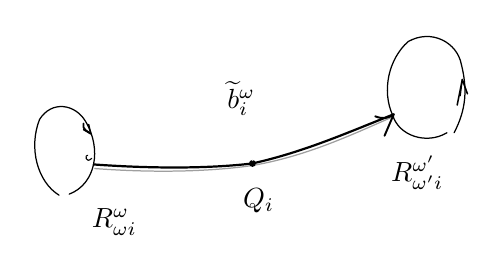
\begin{tikzpicture}[x=.013cm,y=-.013cm,line cap=round,line join=round]
\draw[line width=.45pt] (91,1384) .. controls (70,1371) and (61,1338) .. (72,1310) .. controls (84,1291) and (107,1295) .. (117,1312) .. controls (133,1339) and (127,1373) .. (101,1383);
\draw[line width=.65pt] (115,1314) .. controls (113,1320) and (120,1322) .. (122,1324);
\draw[line width=.55pt] (120,1315) -- (122,1324) -- (115,1320);
\draw[line width=.4pt] (123,1348) .. controls (117,1354) and (116,1344) .. (119,1345);
\draw[line width=.8pt] (125,1354) .. controls (195,1359) and (247,1357) .. (280,1353) .. controls (330,1342) and (375,1322) .. (418,1305);
\draw[line width=.45pt,gray!75] (126,1358) .. controls (193,1363) and (246,1360) .. (280,1355) .. controls (332,1346) and (375,1326) .. (418,1307);
\draw[line width=.7pt] (400,1307) .. controls (408,1310) and (412,1309) .. (418,1305) -- (409,1326);
\fill (280,1353) circle[radius=1.25pt];
\fill[white] (280,1350.3) circle[radius=.2pt];
\draw[line width=.45pt] (470,1323) .. controls (450,1335) and (423,1326) .. (417,1306) .. controls (406,1282) and (413,1251) .. (432,1234) .. controls (455,1221) and (480,1235) .. (484,1256) .. controls (490,1280) and (489,1300) .. (477,1323);
\draw[line width=.55pt] (480,1296) -- (485,1271) -- (490,1285);
\draw[line width=.4pt] (485,1271) -- (483,1287);
\node[above] at (269,1316) {$\widetilde b_i^\omega$};
\node[below] at (286,1368) {$Q_i$};
\node[below] at (145,1388) {$R_{\omega i}^{\omega}$};
\node[below] at (441,1336) {$R_{\omega'i}^{\unsure{\omega'}}$};
\end{tikzpicture}}

On trouve par la commutativité (44) et par la dernière formule (39) qu'on a

\deleted{$\widetilde b_{\unsure{\omega i|\omega\omega\prime}}^{\unsure{\omega}}$}

\[
(45)\qquad\widetilde b_i^\omega\bigl(\psi_i^\omega(\underset{\inserted{x}}{\deleted{\unsure{g}}})\bigr)=\psi_i^{\omega'}\bigl(\sigma_\infty(x).
\]

\margin{63}
